%Version 3 October 2023
% See section 11 of the User Manual for version history
%
%%%%%%%%%%%%%%%%%%%%%%%%%%%%%%%%%%%%%%%%%%%%%%%%%%%%%%%%%%%%%%%%%%%%%%
%%                                                                 %%
%% Please do not use \input{...} to include other tex files.       %%
%% Submit your LaTeX manuscript as one .tex document.              %%
%%                                                                 %%
%% All additional figures and files should be attached             %%
%% separately and not embedded in the \TeX\ document itself.       %%
%%                                                                 %%
%%%%%%%%%%%%%%%%%%%%%%%%%%%%%%%%%%%%%%%%%%%%%%%%%%%%%%%%%%%%%%%%%%%%%

%%\documentclass[referee,sn-basic]{sn-jnl}% referee option is meant for double line spacing

%%=======================================================%%
%% to print line numbers in the margin use lineno option %%
%%=======================================================%%

\documentclass[lineno,sn-basic]{sn-jnl}% Basic Springer Nature Reference Style/Chemistry Reference Style

%%======================================================%%
%% to compile with pdflatex/xelatex use pdflatex option %%
%%======================================================%%

%\documentclass[pdflatex,sn-nature]{sn-jnl}% Basic Springer Nature Reference Style/Chemistry Reference Style


%%Note: the following reference styles support Namedate and Numbered referencing. By default the style follows the most common style. To switch between the options you can add or remove “Numbered” in the optional parenthesis. 
%%The option is available for: sn-basic.bst, sn-vancouver.bst, sn-chicago.bst%  
 
%%\documentclass[sn-nature]{sn-jnl}% Style for submissions to Nature Portfolio journals
%%\documentclass[sn-basic]{sn-jnl}% Basic Springer Nature Reference Style/Chemistry Reference Style
%\documentclass[sn-mathphys-num]{sn-jnl}% Math and Physical Sciences Numbered Reference Style 
%%\documentclass[sn-mathphys-ay]{sn-jnl}% Math and Physical Sciences Author Year Reference Style
%%\documentclass[sn-aps]{sn-jnl}% American Physical Society (APS) Reference Style
%%\documentclass[sn-vancouver,Numbered]{sn-jnl}% Vancouver Reference Style
%\documentclass[sn-apa]{sn-jnl}% APA Reference Style 
%%\documentclass[sn-chicago]{sn-jnl}% Chicago-based Humanities Reference Style

%%%% Standard Packages
%%<additional latex packages if required can be included here>

\usepackage{graphicx}%
\usepackage{multirow}%
\usepackage{amsmath,amssymb,amsfonts}%
\usepackage{amsthm}%
\usepackage{mathrsfs}%
\usepackage[title]{appendix}%
\usepackage{xcolor}%
\usepackage{textcomp}%
\usepackage{manyfoot}%
\usepackage{booktabs}%
\usepackage{algorithm}%
\usepackage{algorithmicx}%
\usepackage{algpseudocode}%
\usepackage{listings}%
%%%%

% I added these packages (QL)
\usepackage{soul}  % to use highlight function
\usepackage{caption}

\renewcommand{\figureautorefname}{Fig.}


% Define a new counter for Extended Data Figures
\newcounter{extendeddatafig}
\renewcommand{\theextendeddatafig}{Extended Data Fig. \arabic{extendeddatafig}}

% Custom command for Extended Data Figures
\newcommand{\extendeddatafigure}[3][]{%
  \refstepcounter{extendeddatafig}%
  \renewcommand{\thefigure}{\theextendeddatafig} % Ensure ref{} uses Extended Data Fig. X
  \begin{figure}[ht]
    \centering
    #2 % Insert figure content (image, plots, etc.)
    \captionsetup{labelformat=empty} % Remove default figure numbering
    \caption{\textbf{\theextendeddatafig}: #1}%
    \label{#3} % Correctly place label after caption
  \end{figure}%
}




%% end of QL's addition
%%%%%=============================================================================%%%%
%%%%  Remarks: This template is provided to aid authors with the preparation
%%%%  of original research articles intended for submission to journals published 
%%%%  by Springer Nature. The guidance has been prepared in partnership with 
%%%%  production teams to conform to Springer Nature technical requirements. 
%%%%  Editorial and presentation requirements differ among journal portfolios and 
%%%%  research disciplines. You may find sections in this template are irrelevant 
%%%%  to your work and are empowered to omit any such section if allowed by the 
%%%%  journal you intend to submit to. The submission guidelines and policies 
%%%%  of the journal take precedence. A detailed User Manual is available in the 
%%%%  template package for technical guidance.
%%%%%=============================================================================%%%%

%% as per the requirement new theorem styles can be included as shown below
%\theoremstyle{thmstyleone}%
%\newtheorem{theorem}{Theorem}%  meant for continuous numbers
%%\newtheorem{theorem}{Theorem}[section]% meant for sectionwise numbers
%% optional argument [theorem] produces theorem numbering sequence instead of independent numbers for Proposition
%\newtheorem{proposition}[theorem]{Proposition}% 
%%\newtheorem{proposition}{Proposition}% to get separate numbers for theorem and proposition etc.

%\theoremstyle{thmstyletwo}%
%\newtheorem{example}{Example}%
%\newtheorem{remark}{Remark}%

%\theoremstyle{thmstylethree}%
%\newtheorem{definition}{Definition}%

\raggedbottom
%%\unnumbered% uncomment this for unnumbered level heads

\begin{document}

\title[Article Title]{Distinct contributions of anterior and posterior orbitofrontal cortex to adaptive decision-making}


\author[1]{\fnm{Qingfang} \sur{Liu}}
\author[2]{\fnm{Daria} \sur{Porter}}
\author[2]{\fnm{Hadeel} \sur{Damra}}
\author[3]{\fnm{Yao} \sur{Zhao}}
\author[1]{\fnm{Geoffrey} \sur{Schoenbaum}}
\author*[1]{\fnm{Thorsten} \sur{Kahnt}}\email{thorsten.kahnt@nih.gov}

\affil*[1]{\orgname{National Institute on Drug Abuse Intramural Research Program}, \orgaddress{\city{Baltimore}, \postcode{21224}, \state{MD}, \country{USA}}}

\affil[2]{\orgdiv{Feinberg School of Medicine}, \orgname{Northwestern University}, \orgaddress{\city{Chicago}, \postcode{60611}, \state{IL}, \country{USA}}}

\affil[3]{\orgdiv{Department of Psychology}, \orgname{University of Pennsylvania}, \orgaddress{\city{Philadelphia}, \postcode{19104}, \state{PA}, \country{USA}}}

%%==================================%%
%% Sample for unstructured abstract %%
%%==================================%%

\abstract{The lateral orbitofrontal cortex (OFC) is critical for flexibly
adjusting choices when outcome values change. This requires
representations of stimulus-outcome associations and inferring the
updated value of outcomes, but whether and how different parts of OFC
contribute to these functions has remained unclear. Here we used
transcranial magnetic stimulation (TMS) to disrupt activity in
functional networks centered on the anterior (aOFC) and posterior (pOFC)
lateral OFC. Participants (n = 48) received aOFC or pOFC network-targeted
TMS either before learning associations between visual stimuli and sweet
or savory food odor rewards, or, on the next day, before a meal to
selectively devalue one of these rewards. TMS targeting pOFC before the
meal disrupted goal-directed behavior, as measured by choices of stimuli
predicting non-sated rewards in a probe test, whereas disrupting aOFC
before learning stimulus-outcome associations similarly impaired choices
in the probe test. These findings demonstrate distinct contributions of
different OFC subregions to goal-directed behavior.}

\keywords{adaptive decision-making, goal-directed behavior, cognitive map, orbitofrontal cortex}

%%\pacs[JEL Classification]{D8, H51}

%%\pacs[MSC Classification]{35A01, 65L10, 65L12, 65L20, 65L70}

\maketitle

\section{Introduction}
\label{sec-intro}

Humans and animals effortlessly adapt to changing environments by flexibly adjusting their behavior. This adaptability relies on outcome-guided decision-making, where individuals can re-evaluate their choices in real time, simulating potential outcomes based on changes in outcome value \citep{RN644} rather than defaulting to habitual responses. For example, a restaurant chef might anticipate that a guest could experience an allergic reaction to certain ingredients and adjust the dish accordingly before an issue arises. To enable this flexibility,
a detailed representation of the environment---commonly referred to as a cognitive map or model-based representation-is essential \citep{behmulwhi18}. A chef with a thorough understanding of ingredient composition and suitable substitutes can efficiently modify recipes to accommodate allergies without compromising the dish. The orbitofrontal cortex (OFC) plays a central role in both processes, supporting adaptive behaviors through the formation of cognitive maps \citep{RN606,RN633} and use the map to simulate potential outcomes \citep{HowRey2020,RN15}. 

Across species, the OFC is known as a heterogeneous region, comprising subregions with varying anatomical and functional properties along both mediolateral and anterior-posterior gradients \citep{RN641,RN640,RN460,RN639,RN531,RN651,RN656,RN657,krirol04,neubert15}. In humans, studies on value-based decision-making have primarily focused on the functional distinctions between the medial and lateral OFC \citep{RN640,RN460,RN656}. However, the anterior-posterior gradient has received less attention, despite anatomical studies in humans and non-human primates revealing a cytoarchitectural progression from granular to agranular cortex along this axis \citep{RN641,RN640,RN657,krirol04,neubert15}.

This study aims to identify the distinct roles of anterior-posterior subregions within the lateral OFC in supporting different aspects of adaptive behaviors in an outcome devaluation task \citep{RN606,HowRey2020,RN645,RN646,RN652,RN530,RN562,RN561,RN632,RN18,RN168,RN647,RN648,RN649}. Outcome devaluation assesses responses to predictive cues following the selective devaluation of the associated outcome, thereby revealing the capacity to align actions with updated goals and contexts. While earlier theories emphasized the role of the OFC in signaling the current value of stimuli to guide response selection \citep{RN652}, more recent and widely supported accounts propose two complementary roles: one in using mental simulations to infer or update the value of outcome-predicting stimuli \citep{RN606,RN530,HowRey2020}, and another in constructing and modifying relevant cognitive map that links stimuli to outcomes during initial learning \citep{RN598}. In the current work, we focus on the latter two mechanims, proposing a unified framework that integrates them within the lateral OFC and empirically tests their distinct predictions regarding functional specialization across subregions.


We hypothesize that disrupting OFC activity during different phases of the outcome devaluation task causes distinct effects on behavior. Specifically, we expect that disrupting the anterior portion of the central/lateral OFC will impair the acquisition of specific stimulus-outcome associations and disrupting the posterior portion will impair retrieving and using these associations to guide choices. To test this, we applied network-targeted transcranial magnetic stimulation (TMS) with continuous theta burst stimulation (cTBS) in a within-participant study across multiple sessions. This approach allowed us to modulate the anterior and posterior portions of the central/lateral OFC network selectively during the learning and testing phases. 

Our findings reveal distinct roles for the anterior and posterior lateral OFC in goal-directed behavior. Disruption of the posterior lateral OFC before testing impaired outcome devaluation, whereas
disruption of the anterior lateral OFC before learning similarly impaired subsequent devaluation. Additionally, cTBS targeting either region disrupted value acquisition, but only during the first session of the within-participant study. Together, these results suggest that anterior and posterior lateral orbitofrontal cortex networks play complementary roles, supporting the acquisition and use of
outcome-specific stimulus-reward associations essential for goal-directed behaviors.




\section{Results}
\label{sec-res}

\subsection{Experimental design and outcome devaluation task.}
\label{subsec-design}


This study follows a within-participant, multiple-session design, with 48 healthy human participants completing a two-day experiment, repeated across three separate sessions (spaced at least one week apart; \autoref{fig-design}A). Each session involves the delivery of either cTBS on one day and sham TMS on the other, or sham TMS on both days, resulting in three conditions (Day 1-Day 2: cTBS-sham, sham-cTBS, sham-sham, order counterbalanced; \autoref{fig-design}D). 

On Day 1, participants learned to discriminate pairs of visual stimuli associated with desirable food odors (sweet or savory, equally valued based on pre-task ratings; \autoref{fig-design}E) and clean air. They were asked to select the stimulus associated with any odor, meaning they were not required to encode the specific stimulus-outcome identity associations to perform the discrimination task (\autoref{fig-design}B, C). On Day 2, participants chose between stimuli based on odor preferences, making choices between stimuli predicting sweet and savory odors, or between stimuli predicting odor and air. A pre-meal free choice task was followed by a meal, then by a post-meal free choice task. Participants received the odors during the Day 1 discrimination task and the Day 2 pre-meal free choice task. No odors were delivered during Day 2 post-meal free choice task. Participants also reported how much they liked each odor before and after the meal. 

To explore the potentially distinct functional roles of OFC subregions in this task, TMS was administered at two different time points---either before the discrimination task on Day 1 or before the meal on Day 2 (\autoref{fig-design}A)---and targeted either the anterior (aOFC) or posterior (pOFC) portions of the lateral OFC in different groups of subjects (\autoref{fig-design}F). Stimulation targets were defined using MNI coordinates in the right hemisphere: aOFC at {[}34, 54, -14{]} and pOFC at {[}28, 38, -16{]}. Each target showed strong functional connectivity with isolated lateral prefrontal cortex (LPFC) ROIs (referred to as aOFC-conn-LPFC and pOFC-conn-LPFC, respectively). Based on resting-state fMRI data from Day 0, we individually selected LPFC stimulation sites
with the highest connectivity to the respective aOFC or pOFC targets (\autoref{fig-design}F). We confirmed the functional separation of these networks across all resting-state fMRI sessions: the aOFC-conn-LPFC showed stronger connectivity with the aOFC than the pOFC ($W = 988$, $p = 1.57e-5$, Wilcoxon signed rank test, two-sided), and the pOFC-conn-LPFC showed stronger connectivity with the pOFC than the aOFC ($W = 936$, $p = 2.23e-4$) (\autoref{fig-design}G).



\begin{figure}
\centering
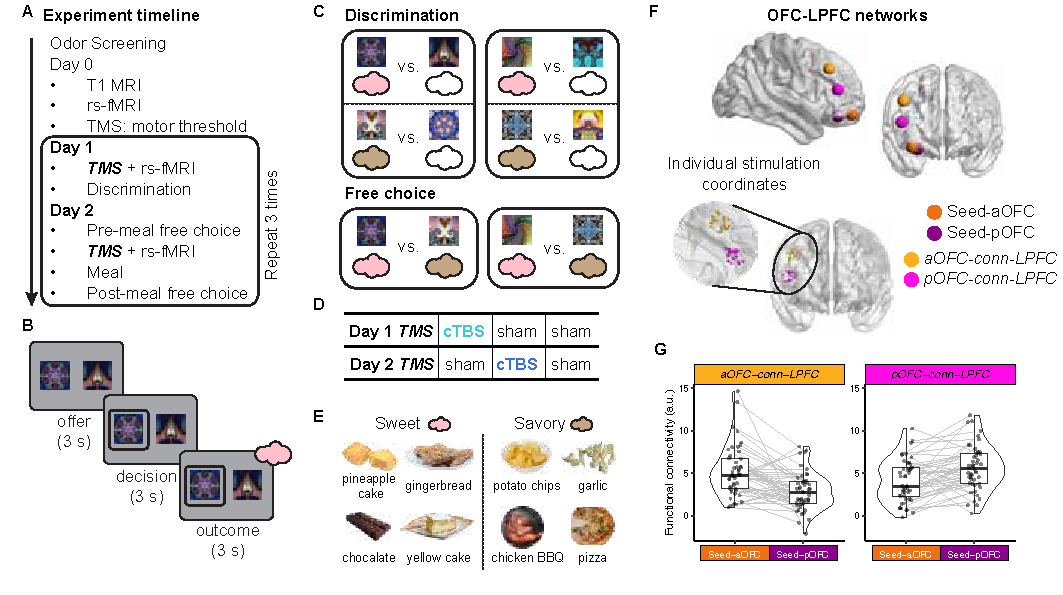
\includegraphics[width=\linewidth]{Fig_design.png}
\caption{\textbf{Experimental design and outcome devaluation task.} \textbf{A. Experiment timeline.} Following odor screening, participants completed T1 MRI, resting-state fMRI, and TMS motor threshold determination on Day 0. On Day 1, they received either continuous theta burst stimulation (cTBS) or sham TMS before a discrimination task. On Day 2, they performed a pre-meal free choice task, received TMS (cTBS or sham), consumed a meal, and then completed a post-meal free choice task. \textbf{B. Trial structure of discrimination and choice tasks.} Each trial started with an offer phase (3 s), presenting two visual stimuli paired with different outcomes, followed by a decision phase (maximum 3 s) where participants selected one stimulus. In the discrimination task, the trial concluded with an outcome phase (3 s) where participants received an odor or no odor, depending on their choice.
\textbf{C. Task structure.} In the discrimination task, participants learned which stimuli predicted odors (colored clouds) versus non-odor (i.e., clean air, empty clouds) outcomes. In the free choice task, participants selected stimuli based on learned odor associations and their odor preference, but without immediate odor delivery. The free choice task also included trials comparing odor-predictive and non-odor-predictive stimuli, similar to the discrimination task. 
\textbf{D. TMS conditions.} Participants were assigned to one of three counterbalanced conditions: (1) cTBS on Day 1, sham on Day 2 (cTBS-sham), (2) sham on Day 1, cTBS on Day 2 (sham-cTBS), and (3) sham on both days (sham-sham). 
\textbf{E. Odor stimuli.} Eight food-related odors (savory and sweet). One savory and one sweet odor was selected per participant to match pleasantness ratings. 
\textbf{F. OFC-LPFC networks.} Stimulation coordinates within LPFC for each participant, selected to maximize functional connectivity with either the aOFC (tangerine) or pOFC (magenta) seed region. 
\textbf{G. Functional connectivity estimates.} Half-violin plots depict distribution of connectivity estimates between stimulated LPFC regions and OFC seed regions. Dots represent individual connectivity estimates, and lines indicate within-subject comparison across different ROI combinations.}
\label{fig-design}
\end{figure}




\subsection{Selective satiation affects free choices.}
\label{subsec-choices}

We conducted a proof-of-concept analysis to determine whether choices on Day 2 were influenced by selective satiation, specifically by feeding participants an odor-matched meal. We examined participants' choices between stimuli predicting sated (SA) and non-sated (NS) odor options in savory-sweet pairs that had not been previously trained. 

Participants' odor pleasantness ratings decreased after the meal across all sessions and participants ($p = 2.75e-13$, \autoref{fig-choices}A). This reduction was unaffected by TMS condition (sham vs. cTBS), TMS target site (aOFC vs. pOFC), session number (1\textsuperscript{st}, 2\textsuperscript{nd}, 3\textsuperscript{rd}), or sated odor type (savory/sweet) (all $p>0.05$; \ref{EDFig_odor}). Importantly, these results suggest that disruption of OFC activity did not impair participants' ability to update the value of reward outcomes \citep{RN454,rhodes13,HowRey2020} 

When collapsing across sessions, post-meal choices of SA stimuli were significantly reduced relative to pre-meal in both the aOFC (Wilcoxon signed rank test, one-sided, $p = 0.024$) and pOFC ($p = 2.3e-3$) groups (\autoref{fig-choices}B), confirming an effect of selective satiation on free choices. SA choices were significantly correlated with the pleasantness difference between sated and non-sated odors, both before and after the meal (\ref{EDfig_choices}A, B), indicating that participants made their choices based on relative odor preference, as anticipated. We further calculated the change in pleasantness for both sated and non-sated odors (post-meal minus pre-meal), and then subtracted the change in non-sated odor ratings from that of sated odors. This ``selective satiation index'' was significantly correlated with the corresponding change in SA choices (Pearson's $r = 0.46$, $p = 8.3e-4$; \ref{EDfig_choices}C), again supporting the behavioral impact of the change of subjective odor value. 

In addition to savory-sweet odor choices, we examined participants’ choices between odors and clean air, which had been associated with outcomes during the Day 1 discrimination task. Participants generally preferred odors over clean air (\autoref{fig-choices}C), consistent with successful learning of odor-outcome associations. 




\begin{figure}
\centering
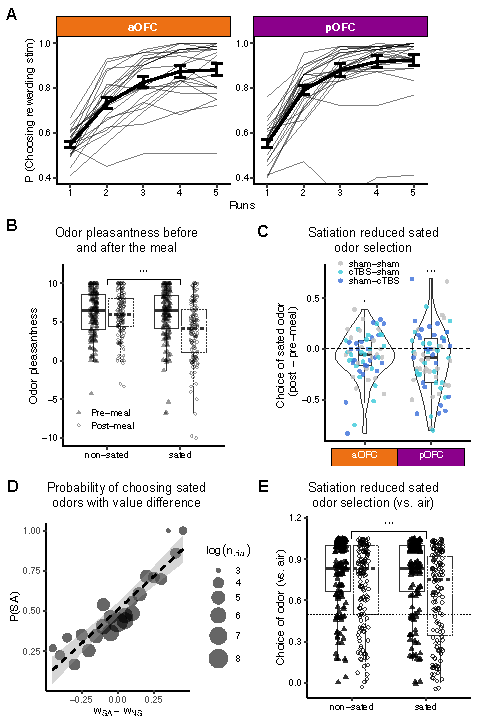
\includegraphics[width=0.85\linewidth]{Fig_choices.pdf}
\caption{\textbf{Selective satiation affects free choices.} 
\textbf{A}. Change of rated odor pleasantness before and after the meal, for sated and non-sated odors. 
\textbf{B.} Choice of sated odors in sweet-savory choices for sham-sham and sham-cTBS conditions, under aOFC-targeted and pOFC-targeted cTBS. 
\textbf{C.} Choice of odors vs. clean air, for sated odors and non-sated odors, pre-meal and post-meal. 
\textbf{D.} Choice of sated odors options with value difference. Dot size represents the number of trials with such value difference. 
}
\label{fig-choices}
\end{figure}


Additionally, although not part of our original hypothesis—and not typically examined in outcome devaluation studies—we found that individual choices were also influenced by the learned value of each stimulus. We estimated these values based on participants' behavior during the Day 1 discrimination task (see Section \ref{subsec:disc} for details). The probability of choosing the SA option significantly increased with the value difference between the two stimuli ($w_{SA}-w_{NS}$)  (Pearson's $r = 0.92$, $p = 3.49e-10$; \autoref{fig-choices}D, \ref{EDfig_choices}D).

Therefore, when evaluating the effects of cTBS (applied on Day 1 or Day 2) on SA choices during Day 2, we included both the learned value difference ($w_{SA}-w_{NS}$) and the selective satiation index as regressors to account for factors influencing behavior beyond the effects of TMS. 



\subsection{Posterior, but not anterior, OFC-targeted cTBS before the free choice  impairs outcome devaluation}
\label{subsec-day2}

To examine the role of the aOFC and pOFC in outcome devaluation during the test phase, we focused on the ``sham-sham'' and ``sham-cTBS'' TMS conditions. We found a significant interaction between stimulation location (aOFC vs. pOFC targeting) and TMS condition (sham vs. cTBS on Day 2, Day 1 fixed at sham) in predicting SA choices ($p = 0.00548$), according to logistic mixed-effects models on post-meal SA choices, with the session odor preference baseline, satiation status, and the value difference ($w_{SA}-w_{NS}$) accounted for. We further separately analyzed the aOFC and pOFC group  (\autoref{fig_day2}A) and found that cTBS significantly increased SA choices --- indicating poorer adaptation to the current goal --- only in the pOFC group ($p = 0.00036$), but not in the aOFC group ($p = 0.655$). Additionally, we confirmed that the effect of pOFC-targeted cTBS on SA choices remained robust regardless of session order (\ref{EDFig_day2}B). 

We conducted additional analyses to assess whether the effect of TMS on SA choices was driven by other factors, such as satiation status or perceived TMS discomfort or intensity. The across-participant correlations between pleasantness ratings and SA choices were unchanged by Day 2 cTBS (all $p > 0.05$; \ref{EDfig_choices}C), suggesting that the effect of day 2 cTBS on SA choices was not modulated by satiation status. Moreover, the changes in sated odor choices induced by cTBS could not be explained by perceived TMS discomfort or intensity, as incorporating TMS ratings into the regression models did not alter any of the findings (\ref{EDFig_corr}).


We also examined choices made between an odor and clean air to see if TMS had any effect on those choices. Following the meal, preference for sated odors (vs. clean air) decreased, while choices for non-sated odors (vs. clean air) remained unchanged. This decrease in sated odor selection was significantly stronger after sham stimulation (Wilcoxon signed-rank test, $p = 0.018$, two-sided) but not after cTBS on Day 2 ($p = 0.91$; \ref{EDFig_day2}B). SA choices were marginally lower after sham compared to cTBS but only with pOFC targeting ($p = 0.06$) and not aOFC ($p = 0.43$; \autoref{fig_day2}B). These findings align with results from savory-sweet choices, indicating that pOFC-targeted cTBS on Day 2 also impaired choice updating for non-sated odors. This strengthened the critical role of pOFC for adaptive decision-making, even in previously well learned trials.

Together, this suggests that pOFC-targeted cTBS before the free choice phase impaired outcome devaluation, as indicated by an increase of selecting sated odor-predicting stimuli. In contrast, aOFC-targeted cTBS had no such effect, highlighting the specificity of the pOFC involvement. 


\begin{figure}
\centering
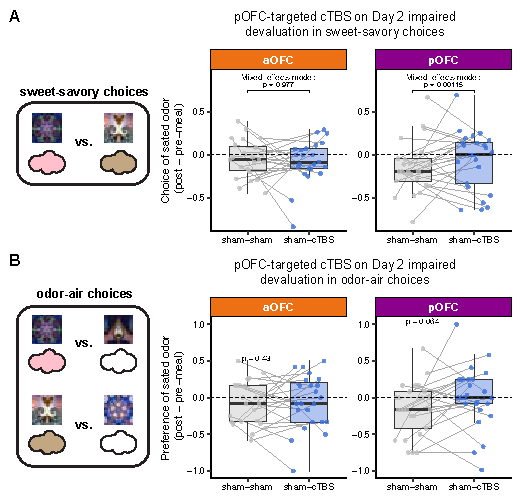
\includegraphics[width=0.85\linewidth]{fig_day2.pdf}
\caption{\textbf{Posterior, but not anterior, OFC-targeted cTBS before the free choice  impaired outcome devaluation}. 
\textbf{A.} Change of choice of sated odors in sweet-savory choices from pre-meal to post-meal test. 
\textbf{B.} Change of preference of sated odors relative to non-sated odors, by comparing odor choices between odor vs. clean air. }
\label{fig_day2}
\end{figure}


\begin{figure}
\centering
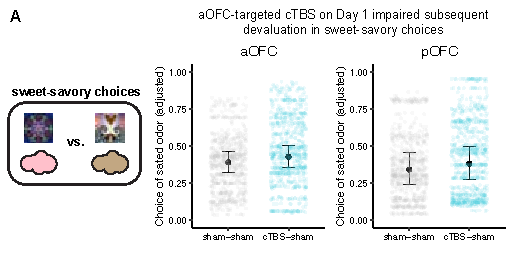
\includegraphics[width=0.85\linewidth]{fig_day1.pdf}
\caption{\textbf{Anterior, but not posterior, OFC-targeted cTBS on Day 1 impaired subsequent devaluation behaviors}.
\textbf{A}. Probability of sated odor selection after the meal, after adjusting modeled contributions of value difference, selective satiation effects, pre-meal odor preference, compared between sham-sham and cTBS-sham sessions. Overlayed points are the model fitted values of the sated odor selection for each trial collapsing across participants. 
}
\label{fig-day1}
\end{figure}


\subsection{Anterior, but not posterior, OFC targeted cTBS before discrimination learning impaired subsequent outcome devaluation}
\label{subsec-day1}

We explored whether cTBS targeting aOFC and pOFC before learning could affect outcome devaluation measured on Day 2, as would be expected if cTBS disrupted the learning of stimulus-reward identity. We predicted that aOFC-targeted cTBS disrupts the latent learning of reward identity.

To assess Day 1 cTBS effect on post-meal choices of sated odors on sweet-savory choices, we focused on ``sham-sham'' and ``cTBS-sham'' TMS conditions. For the aOFC group, both TMS condition and session number significantly influenced post-meal sated odor choices, with a significant interaction between the two. Specifically, the cTBS-sham condition significantly increased the selection of sated odors (\autoref{fig-day1}A; $\hat{\beta} = 1.527$, SE = 0.625, $p=0.015$), and this effect diminished over sessions ($\hat{\beta} = -0.657$, SE = 0.290, $p=0.024$). Choices also increased with session number ($\hat{\beta} = 0.550$, SE = 0.165, $p=8.5e-5$). Additional covariates, including selective satiation index, value difference, and pre-meal odor preference, were significant predictors. Overall, aOFC-targeted cTBS on Day 1 increased post-meal choices of stimuli predicting sated odors, with the effect moderated by session number. For the pOFC group, similar analyses revealed no significant difference between the sham-sham and cTBS-sham stimulation conditions, regardless of whether session numbers were considered as a covariate (\autoref{fig-day1}A; all $p>0.05$). However, pre-meal odor preference and value difference were significant predictors of post-meal choices, while the selective satiation index was not ($p>0.05$). Additionally, no interaction between stimulation location and TMS condition was identified ($p>0.05$). 


These findings support our hypothesis that the aOFC plays a critical role in specific stimulus-outcome learning on Day 1, even when the task does not require it. Notably, this result is independent of the Day 2 TMS, emphasizing the aOFC's importance in constructing cognitive maps that are later used to guide behavior. 


\subsection{Posterior, or anterior, OFC-targeted cTBS disrupted value acquisition, only when applied during the first session}
\label{subsec:disc}

The discrimination task on Day 1 required participants to select the stimulus associated with desirable food odors (vs. clean air) from a pair of stimuli, reflecting a process of value acquisition. Over five runs, participants significantly improved in selecting odor-predictive stimuli ($p<2.2e-16$). This improvement was influenced by both the TMS condition applied before the task (cTBS vs. sham; $p = 1.27e-07$) and the session number (1\textsuperscript{st}, 2\textsuperscript{nd}, 3\textsuperscript{rd} session; $p = 1.71e-11$), and their interaction ($p = 1.93e-5$), according to logistic mixed-effects models with participants as a random factor (Line plot and error bar, \autoref{fig_disc}A). Response times decreased significantly across runs ($p<2.2e-16$), where this decrease was affected by session number ($p<2.2e-16$, \ref{EDFig_disc}A) but was not by TMS condition ($p = 0.541$), according to linear mixed-effects models with participants as a random factor.

To further examine the contributions of TMS condition and session number to discrimination behavior, we grouped participants by the order in which they received cTBS or sham on Day 1 (\autoref{fig_disc}B). This analysis revealed that the impairment in discrimination due to cTBS was only observed when cTBS was applied during the first session ($p<2.2e-16$). We additionally investigated whether the effect of cTBS varied depending on whether stimulation targeted the anterior or posterior OFC but found no evidence suggesting a differential effect (all $p>0.05$).

To quantify and compare the learning process, we fitted a Rescorla-Wagner model to the discrimination behavior using a hierarchical Bayesian approach \citep{RN630} (see \textbf{Supplementary Note} for details). We compared three models: one with condition-specific learning rates, one with session-specific learning rates, and one with fixed learning rates across sessions/conditions. Model comparison showed that the session-specific learning rate model provided the best fit (deviance information criterion \citep{RN159}; DIC; session-specific learning rates = 13161.95, condition-specific learning rates = 13544.84, fixed learning rates = 14045.46). The winning model well captured the data, as illustrated by the shaded fit overlaid on the experimental data (\autoref{fig_disc}A). We examined the estimated learning rates from the winning model and compared them across TMS conditions for each participant group. Wilcoxon signed-rank tests revealed that learning rates were significantly lower after cTBS compared to sham, but only for participants who received cTBS during their first session ($p = 0.0027$; \ref{EDFig_disc}B). We explored if the low learning rates in this group were correlated with perceived TMS discomfort and intensity reported by the participants (\ref{EDFig_disc}C) but found no significant correlation ($r = -0.12$, $p = 0.65$).

Overall, cTBS targeting both posterior and anterior OFC impaired value acquisition in the discrimination task, but only when applied during the first session. This likely reflects participants' initial difficulty in performing the task due to cTBS. As noted in the earlier sections of the results, we included the estimated difference in learned values as regressors when assessing the effects of cTBS (Day 1 or Day 2) on Day 2 choices when estimating cTBS effects on SA choices. 

\begin{figure}
\centering
\includegraphics[width=0.7\linewidth]{fig_disc.pdf}
\caption{\textbf{Posterior or anterior OFC-targeted cTBS disrupted value acquisition, when applied during the first session.} \textbf{A. Discrimination accuracy across runs}. This is plotted by day 1 TMS conditions (cTBS, sham), and session numbers (1\textsuperscript{st}, 2\textsuperscript{nd}, 3\textsuperscript{rd}), separated by different OFC targeted locations (aOFC, pOFC). Line plots and error bars display the experimental data while the shade displays the 95\% confidence interval of simulated accuracy using the posterior estimates of learning rates. 
\textbf{B.} Discrimination accuracy across runs, separated by session numbers and the session order of Day 1 TMS.}
\label{fig_disc}
\end{figure}




\section{Discussion}
\label{sec:discuss}

In this study, we used a three-session times two-day design with network-targeted TMS to selectively modulate activity in anterior and posterior subregions of the human lateral OFC. Using an outcome devaluation task requiring adaptive decision-making based on learned stimulus-outcome identity associations, we found that TMS targeting the pOFC (but not the
aOFC) prior to the meal disrupted adaptive behavior, as evidenced by increased choices of stimuli predicting non-sated rewards in the probe test. Conversely, disrupting the aOFC (but not the pOFC) before learning stimulus-outcome associations impaired behavior in the probe test on the following day. These findings demonstrate that the aOFC facilitates
adaptive decision-making by supporting the acquisition of stimulus-outcome associations, while the pOFC supports their use.



Our findings suggest that the anterior OFC plays a key role in enabling individuals to explore specific stimulus-outcome structures (e.g., associating visual stimuli with specific odors) even when the current task did not explicitly require it. This aligns with prior work indicating that the OFC represents the current state in a state space
\citep{RN606,RN643}. However, our study has some nuanced conceptual difference as the stimulus-outcome associations were directly observable, contrasting with partially observable problems where states cannot be directly observed from perceptual features in the task environment, and often require using retained information in the memory or inferred \citep[e.g.][]{RN642,RN457}. The cognitive map representation function of the anterior OFC identified here bear more resemblance to previous research indicating that both humans and animals are driven by curiosity to explore and learn about the environment, known as latent learning \citep{RN633,RN592}, constructing a representation of the world even in the absence of direct rewards \citep{RN633,RN614,RN634}.
Such cognitive maps, once formed, provide a foundation for guiding
goal-directed behaviors \citep{behmulwhi18,RN592}. In that sense, this work draws important parallel with the rodent study where it shows that chemogenetic inhibition of lateral OFC caused a deficit in credit assignment during map construction \citep{RN598}. Notably, our findings highlight the specific and causal role of the anterior lateral OFC among large area of the OFC in supporting this map formation process. This work is also in line with recent studies in both rodents and humans that suggest that the lateral OFC plays a specific role in learning the identity of rewards associated with stimuli
\citep{RN598,RN30,RN28,liuyaoatt24,RN650,RN451}. However, the current study offers a
novel and unique contribution by showing that aOFC remains essential even when individuals are not explicitly tasked with encoding such identity information. Moreover, when identity encoding is impaired, the deficit extends to later stages, where the encoded information is crucial for adaptive decision making.

Consistent with previous work \citep{HowRey2020}, we found that the posterior OFC is critical for goal-directed behavior. Without an intact posterior OFC, individuals fail to update stimulus choices after selective satiation, continuing to choose stimuli predicting devalued outcomes. This suggests that the posterior OFC may support retrieving and applying the cognitive map to guide behavior. Additionally, disrupting the pOFC before testing impaired value-based stimulus selection.

Our findings align with a range of studies demonstrating distinct roles of OFC subregions across various tasks and across species, including goal-directed choices with outcome devaluation \citep{RN530}, two-choice probabilistic tasks \citep{RN636}, differential information encoding in the OFC \citep{RN637}, and the specific contributions of central OFC subregions to economic decision-making \citep{RN531}. Particularly relevant is work in non-human primates examining the differential roles of OFC subregions in flexible behavior \citep{RN530}, demonstrating that the anterior OFC (area 11) is more involved in goal selection during choice, while the posterior OFC (area 13) primarily supports outcome value updating. Different from \cite{RN530}, our study focuses on differential involvement of lateral OFC subregions in representing and using stimulus-outcome identity associations to guide adaptive behavior. While precise cross-species mapping of our defined anterior and posterior OFC regions to animal models remains challenging, our study is, to our knowledge, the first human investigation to differentiate the functional roles of the OFC along the anterior-posterior gradient in goal-directed and adaptive decision-making. Recognizing these functional differences is crucial to prevent oversampling or undersampling specific regions when assessing the OFC’s role in learning and decision-making. In human research, this distinction is particularly important for neuroimaging studies and neuromodulation approaches targeting the OFC \citep{RN168,HowRey2020,liuyaoatt24,RN4,RN564,oue15}.

Although not part of our initial hypothesis, we found that cTBS targeting both the anterior and posterior OFC disrupted discrimination task performance, but only during the first session, with no impact in later sessions. This challenges the common view that OFC is not essential for simple Pavlovian acquisition \citep{RN654,del07}. However, some rodent studies also suggest that OFC's role in Pavlovian acquisition may be more nuanced than previously thought \citep{RN653}. Interpreting this result is further complicated by our within-participant design, as the deficit emerged only in the first session. This impairment likely reflects initial difficulty in grasping the task's basic structure. Once this fundamental task structure is learned, it can be reused in subsequent sessions with different stimulus sets \citep{behmulwhi18,RN635}, potentially explaining why an intact lateral OFC less critical to task performance in later sessions. Accordingly, we included the stimulus-level learned value of each option in the analysis of SA choices, instead of simply assuming ``perfect" learning of the value from the discrimination learning \citep{RN530,HowRey2020}.


One limitation of this study is the within-participant design, which enhances statistical power but may introduce interpretive challenges. For instance, participants completing the first session could learn that odor identity would be relevant for the Day 2 task, potentially altering their approach to processing odor identity in later sessions. To mitigate this, we compared groups of participants based on the order of cTBS and sham stimulation. Importantly, no findings were driven by stimulation order, speaking to the robustness of our results. However, the small sample size within each order group may limit the detection of subtle order effects. Another limitation is the difference in perceived TMS discomfort and intensity between cTBS and sham conditions as reported in current work and our previous work \citep{liuyaoatt24}. However, our analyses found no differences in these ratings between anterior and posterior sites, and they did not account for the observed behavioral effects. 

\section{Conclusion}
\label{sec-conc}

In conclusion, our study reveals distinct roles of the anterior and posterior OFC in cognitive map formation and its use in an outcome devaluation task in humans. These findings contribute to a deeper understanding of OFC subregions in adaptive decision-making. Additionally, this work offers valuable insights for research in rodents and non-human primates, advancing our understanding of the neural mechanisms underlying adaptive decision-making across species.



\section{Methods}
\label{sec:method}
\subsection{Participants} 
\label{participants}

Eighty-eight healthy, right-handed participants (ages 18-40) with no history of psychiatric or neurological disease provided written informed consent to participate in this study. Of these, 48 participants (16 males; ages 18-40, mean = 25.17, SD = 4.14) completed all sessions. Due to a technical error, behavioral data from the cTBS-sham session were unavailable for one participant, but data from the other two sessions were included in the analysis where applicable. MRI data for five resting-state scans were not acquired and were excluded from analysis. All participants fasted for at least four hours before each study visit.


\subsection{Study design} 
\label{study-design}

The study consisted of eight visits (\autoref{fig-design}A, D), with Day 1 and Day 2 occurring consecutively and repeated across three sessions. Sessions were spaced at least one week apart, with a median interval of 13.5 days, a mean of 18.02 days (SD = 9.09), and a range of 7 to 63 days. On each Day 1 and Day 2, participants received either continuous theta-burst stimulation (cTBS, labeled C) or sham stimulation (S). Over the three sessions, they experienced three TMS conditions: cTBS-sham (CS), sham-cTBS (SC), and sham-sham (SS). The order of these conditions was counterbalanced, with 9 participants receiving CS-SC-SS, 7 receiving CS-SS-SC, and the remaining 32 equally assigned to one of the other four possible sequences.

To prevent differences in stimulation location from affecting participants' experience across sessions, each participant received TMS targeting either the anterior or posterior portion of the lateral OFC throughout all three sessions. Among the participants, 16 of 32 females and 9 of 16 males received TMS targeted to the posterior portion. Additionally, the order of satiation conditions was counterbalanced: half of the participants received a sweet meal in their first session, while the other half received a savory meal. The sated odor type alternated for each participant across the three sessions (e.g., savory-sweet-savory or
sweet-savory-sweet).

\subsection{Screening session}
\label{screening-session}

After providing informed consent and completing eligibility screening, participants rated the pleasantness of eight food odors. These odors, supplied by International Flavors and Fragrances (New York, NY), included four savory (garlic, potato chip, pizza, barbecue) and four sweet (chocolate, yellow cake, pineapple cake, gingerbread) odors. In each trial, participants smelled a food odor for 2 seconds and rated their liking on a visual analog scale ranging from ``Most Disliked Sensation Imaginable'' to ``Most Liked Sensation Imaginable.'' Ratings were made using a scroll wheel and keyboard press. Each odor was presented three times in a pseudo-randomized order, and ratings were averaged per odor. Based on these ratings, two odors (one savory, one
sweet) that were pleasant (above neutral) and closely matched were selected for the discrimination and choice tasks. These odors were used across all three sessions. Participants were excluded if no suitable odors were identified.

A custom-built, computer-controlled olfactometer was used to deliver the
odors with precise timing to nasal masks worn by participants. The
olfactometer directed medical-grade air through the headspace of amber
bottles containing the odor solutions at a constant flow rate of
3.2L/min. Using two independent mass flow controllers (Alicat, Tucson,
AZ), the device enabled precise dilution of the odorized air with
odorless air. Throughout the experiment, a constant stream of odorless
air was delivered, and odorized air was mixed in at specific time points
without altering the overall flow rate or causing somatosensory
stimulation.

\subsection{Day 0: Scan \& Motor threshold} 
\label{day-0-scan-motor-threshold}

We acquired a T1-weighted structural MRI scan to assist with TMS neuronavigation and an 8 min multi-echo resting-state fMRI scan (310 volumes, TR = 1.5s) to individually define the OFC-targeted cTBS coordinates (see section \ref{coordination-selection}). The same scanning parameters were used for
other resting-state scans. We then measured resting motor threshold (rMT) by administering single TMS pulses to the hand area of the left motor cortex. rMT was defined as the lowest percentage of stimulator output required to evoke 5 visible thumb movements from 10 pulses.

\subsection{Day 1: Discrimination task} 
\label{day-1-discrimination-task}

Participants first underwent a TMS session (cTBS or sham, see section \ref{tms}) followed by a resting-state scan. Then they completed five runs of a discrimination task. In each trial, participants chose between two
fractal stimuli: one associated with a savory or sweet odor, and the
other with clean air. Stimuli were displayed for 3 seconds, followed by
a choice phase (maximum 3 seconds). If participants selected a stimulus
leading to an odor, the odor was delivered for 2 seconds. The
inter-trial interval ranged from 4 to 8 seconds. Each run consisted of
24 trials, using four groups of stimulus pairs: two sets (A and B)
crossed with sweet/savory odors. Each combination had three
non-overlapping stimulus pairs, resulting in 24 distinct fractals. Each
pair was presented twice to counterbalance left and right positions.
Choice and response times were recorded for each trial, and different
fractals were used across the three sessions.


\subsection{Day 2: Meal consumption and free choice task} 
\label{day-2-meal-and-choice}

Day 2 started with an odor pleasantness rating followed by a choice task (pre-meal) where participants selected between pairs of stimuli. Afterwards, participants underwent a TMS session and then had a meal carefully matched in flavor to either the sweet or savory food odor used in their task. Following the meal, participants completed another set of odor pleasantness ratings and the post-meal free choice task. Both pre-meal and post-meal choice tasks instructed participants to choose based on their current odor preferences. In the pre-meal free choice task, participants received the odor associated with their selected stimulus. In the post-meal free choice task, no odors were delivered immediately, but participants were told that five randomly selected trials would result in odor delivery at the end of all trials.

The pre-meal free choice task included 30 trials, all from set A, consisting of 3 sweet vs. clean air pairs, 3 savory vs. clean air pairs, and 9 savory vs. sweet pairs. Each pair was presented twice to counterbalance left and right positions. The post-meal choice task included 60 trials from both sets A and B. In both pre- and post-meal choice tasks, similar to the discrimination task, every trial began with a pair of stimuli presented for 3 seconds, followed by a decision phase of up to 3 seconds. In the pre-meal free choice task, if participants selected a stimulus linked to an odor, the odor was delivered for 2 seconds after their choices. In the post-meal free choice task, five odors were delivered, each for 2 seconds, after all trials were completed. The inter-trial interval ranged from 4 to 8 seconds, and choice and response times were recorded from all trials. Pre- and post-meal free choices for both set A and set B stimuli were highly correlated (\ref{EDFig_sets}), indicating consistent choices across sets based on odor preferences. Thus, to assess the satiation effect on choices, we used the pre-meal average choice from set A as a session-wise odor preference baseline and compared it with the post-meal choices.

\subsection{MRI data acquisition} 
\label{mri-data-acquisition}

Each TMS session on Day 1 and Day 2 was immediately followed by a
resting-state MRI scan. MRI data were acquired on a Siemens 3T PRISMA
system equipped with a 64-channel head-neck coil. Resting-state fMRI
data were collected across all seven sessions with the same multi-echo
sequence (310 volumes; TR = 1.5s; TE1-TE3 = 14.60ms, 39.04ms, 63.48ms).
The short TE of the first echo is beneficial to mitigate signal dropout
near the OFC, as demonstrated in previous studies using both resting-state and task-based fMRI \citep{RN619,RN524,kirlutpos16,zhao24img}. Other scanning parameters included: flip angle, 72°, slice thickness, 2mm (no gap), multi-band acceleration factor 4, 60 slices with interleaved acquisition, matrix size 104 x 104 voxels, and field of view 208mm x 208mm. A 1mm isotropic T1-weighted structural scan was acquired on Day 0 session for neuronavigation during TMS and to aid spatial normalization.

\subsection{Coordination selection for network-targeted TMS} 
\label{coordination-selection}

The stimulation coordinates were computed based on the multi-echo resting-state MRI data collected from the Day 0 session. We defined our stimulation targets in the right hemisphere's aOFC and pOFC using MNI coordinates: aOFC {[}34, 54, -14{]} and pOFC {[}28, 38, -16{]}. The pOFC coordinates were identical to those used in our previous network-targeted TMS studies \citep{HowRey2020,liuyaoatt24,RN4,RN564}, which have been found to correlate with the identity of reward outcomes \citep{HowRey2020,RN4}. Each targeted coordinate in the aOFC and pOFC exhibited strong functional connectivity with separate LPFC clusters with peak coordinate of {[}44, 28, 38{]} and {[}46, 38, 14{]}, respectively. This functional connectivity was determined based on a meta-analysis from Neurosynth.org involving a sample of 1,000 subjects. We first generated spherical masks of 8-mm radius around these four coordinates in MNI space, each inclusively masked by the gray matter tissue probability map provided by SPM12 (thresholded at \textgreater{} 0.1). We then transformed these four masks to each subject's native space using the inverse deformation field generated during the normalization of the T1 anatomical image. We then specified two resting-state fMRI functional connectivity analyses (one per region) for each subject, using individual OFC masks as the seed region and motion parameters from the realignment of the first echo as regressors of no interest. Finally, stimulation coordinates were defined as the voxels within the right LPFC masks with the strongest functional connectivity to the right aOFC and pOFC seed regions, respectively. We used infrared MRI-guided stereotactic neuronavigation (LOCALITE) to apply stimulation to these two individual LPFC coordinates.

\subsection{Transcranial magnetic stimulation} 
\label{tms}

Similar to our previous work, the target coordinates were defined as the locations in the right LPFC with the strongest functional connectivity with the corresponding right OFC seed regions (see details above). The Figure-eight coil was tilted so that its long axis was approximately perpendicular to the long axis of the middle frontal gyrus. TMS was administered at 80\% of the rMT using a cTBS protocol. This protocol involved delivering bursts of three pulses at 50 Hz every 200 ms (5 Hz) for a total of 600 pulses over approximately 40 seconds. Stimulation was applied using a MagPro X100 stimulator equipped with a MagPro Cool-B65 A/P butterfly coil (MagVenture). Previous work has demonstrated that this cTBS protocol at 80\% MT has inhibitory aftereffects which persist for 50–60 min over primary motor cortex \citep{RN51}. Whereas cTBS was delivered by positioning the active side of the A/P coil to modulate neural tissue, sham cTBS was applied with the placebo side of the A/P coil, producing similar somatosensory and auditory experiences for the participant without modulating neural tissue. Electrodes were placed on participants' forehead and direct current stimulation was applied in synchrony with the TMS pulses to mask TMS effects and enhance the similarity between cTBS and sham sessions.

Participants were informed about potential muscle twitches in the face, eyes, and jaw during simulation. To assess tolerability, two
single pulses were applied over the stimulation coordinates before
administering cTBS. Discomfort and perceived stimulation intensity were evaluated after each TMS session. The cTBS session was generally rated as more uncomfortable and intense compared to the sham session. On a scale from 0 (not uncomfortable at all) to 10 (extremely uncomfortable), mean discomfort ratings were 3.38 for
sham and 5.8 for cTBS sessions ($p=2.2e-16$, linear mixed effects
model). Similarly, on a scale from 0 (not strong at all) to 10 (extremely strong), mean intensity ratings were 3.79 for sham and 6.23 for cTBS sessions ($p=2.2e-16$, linear mixed effects model). Discomfort and intensity ratings did not differ between aOFC- or pOFC-targeted cTBS (all $p>$ 0.6). For analyses involving cTBS effects (Day 1 or Day 2 TMS), standardized discomfort and intensity ratings were used to examine correlations or regressions against other variables, assessing if the observed cTBS effects were driven by subjective discomfort or perceived TMS intensity, but none of the effects can be explained by those ratings (see \ref{EDFig_corr}).



\subsection{Meal consumption} 
\label{meal-consumption}

On Day 2, participants consumed a meal following the TMS session to selectively satiate one of the two food odors. The meal items were carefully chosen to closely match the corresponding food odors, and water was provided. Participants were instructed to eat until they
felt very full and were then left alone for 15 minutes. Immediately afterward, they rated the pleasantness of the odors and
proceeded to the post-meal choice task. On average, participants consumed 669.89 ± 44.16 calories (SEM). Before analyzing the relationship between odor ratings and task behavior, we standardized the ratings within each participant across sessions. 


\subsection{Modeling value learning process} 
\label{modeling-value-learning}

We used a standard Rescorla-Wagner model \citep{RN520} to describe learning in the discrimination task, where participants chose between two stimuli—one predicting an odor and the other leading to clean air. Since stimulus pairs had no overlap, we assumed that learning was primarily driven by the odor-predictive stimulus rather than the stimulus associated with clean air. Accordingly, we modeled the learned value $v$ of the odor-predictive stimulus across trials.

The model updated $v$ of the odor-predictive stimulus based on prediction error, defined as the difference between the actual outcome ($v=1$) and the expected value on each trial. The learning rate determined how quickly $v$ adjusted across trials. Initially, $v$ was set to 0.5, with $v=1$ indicating complete learning of the odor-predictive stimulus. We estimated a separate learning rate for each odor-predictive stimulus, with priors constrained by session-wise or condition-wise hyper parameters in a hierarchical Bayesian framework \citep{RN630}. This approach allowed us to obtain learned value estimates for each odor-predictive stimulus, which were then used to aid the analysis of the free-choice task data. 
The session-wise hyper learning rate parameters are used to correlated with TMS ratings in \ref{EDFig_disc}. Details of the model specification and estimation are provided in \textbf{Supplementary Text 1.}


\subsection{Multi-echo MRI data processing}
\label{multi-echo}

Preprocessing of the multi-echo resting-state fMRI data involved several
steps. First, all functional images from the smallest echo across all
rs-fMRI runs were realigned to the first volume of the first echo, and
the resulting voxel-to-world mapping matrix was applied to the other two
echoes, volume by volume. All functional images were then resliced for
each echo. Next, the images in each echo were combined using temporal
signal-to-noise ratio (tSNR) weighting, following parallel-acquired
inhomogeneity desensitized (PAID) approach \citep{RN524}. Specifically, voxel-wise tSNR maps were computed for each echo, multiplied by the echo time (TE), and normalized across the three echoes to generate weight maps. These weight maps were then used to combine the resliced images by multiplying each volume by its respective weight map. Lastly, the combined data underwent coregistration, normalization, and
smoothing using a 6 mm FWHM Gaussian kernel.

We analyzed participants' motion during the resting-state scan after different types of TMS (sham vs. cTBS) and stimulation targeted locations (anterior vs. posterior OFC). Framewise displacement (FD) was calculated per volume and summed across volumes \citep{RN521}. No significant differences were observed between TMS types or stimulation locations (all $p>$ 0.8). FD for cTBS was 38.3mm (±10.8mm) at the anterior OFC and 41.3mm (±17.8mm) at the posterior OFC, while for sham, FD was 41.0mm (±16.7mm) at the anterior OFC and 39.6mm (±15.8mm) at the posterior OFC.



\backmatter


\bmhead{Acknowledgements}

We thank Dr. Geoffrey Schoenbaum and Dr. Yihong Yang for their helpful discussions. This work was supported by National Institute on Deafness and Other Communication Disorders grant R01DC015426 (to T.K.) and the Intramural Research Program at the National Institute on Drug Abuse (ZIA DA000642, to T.K.). The opinions expressed in this work are the authors’ own and do not reflect the view of the NIH/DHHS.


\section{Extended Data}
\label{sec-EDFig}



\extendeddatafigure[
\textbf{Supplementary results on odor pleasantness ratings.} 
\textbf{A.} Odor pleasantness ratings separated by TMS conditions and stimulation locations. 
\textbf{B.} Odor pleasantness ratings separated by session numbers and stimulation locations.
]{
\includegraphics[width=0.7\linewidth]{EDfig_odor.pdf}
}{EDFig_odor} 





\extendeddatafigure[
\textbf{Free choices are influenced by learned stimulus values and selective satiation effects.} 
\textbf{A.} Scatter plots showing correlations between the choice of sated odors and odor preference before and after the meal, separated by the three TMS conditions. 
\textbf{B.} Scatter plot showing the change in SA choices against the change of odor pleasantness difference after eating the meal. 
\textbf{C.} Choice of sated odors options associated with each of the learned weight of the combination of sated and non-sated options. Dot size represents the number of trials per value combination (log scale), with missing dots indicating unobserved combinations. 
]{
\includegraphics[width=0.7\linewidth]{EDfig_choices.pdf}
}{EDfig_choices}



\extendeddatafigure[
\textbf{Scatter plots showing high correlations of the choice for selecting sated odors across post-meal, pre-meal, set A and set B. } 
\textbf{A.} Relationship between pre-meal and post-meal of set A.
\textbf{B.} Relationship between pre-meal and post-meal of set B.
\textbf{C.} Relationship between pre-meal set A and post-meal of set B.
]{
\includegraphics[width=0.7\linewidth]{EDfig_sets.pdf}
}{EDFig_sets} 




\extendeddatafigure[
\textbf{Relationship between perceived TMS discomfort and intensity and sated odor (SA) choices.}
\textbf{A.} Correlation between SA choices and TMS ratings, separated by Day 2 TMS conditions (sham-cTBS vs. sham-sham) and TMS targeted regions (aOFC, pOFC). A positive correlation was observed between TMS ratings and SA choices in the aOFC group, but including ratings of TMS perception into the regression models did not alter the observed TMS effects on SA choices.
\textbf{B.} Same as \textbf{A}, but focus on Day 1 TMS effect (sham-sham vs. cTBS-sham).
\textbf{C.} Scatter plot showing the relationship between the condition-wise difference (sham-cTBS vs. sham-sham) of SA choices and condition-wise difference of TMS ratings from Day 2 TMS. There was a significant positive correlation in the aOFC group (Pearson's $r = 0.7$, $p = 7.9e-8$)
\textbf{D.} Same as \textbf{B}, but focus on Day 1 TMS effect (sham-sham vs. cTBS-sham).
Shaded areas represent 95\% confidence intervals estimated using robust linear regression. Marginal distributions are shown on the top and right axes. Pearson correlation coefficients (R) and p-values are reported for each TMS condition.
]{
\includegraphics[width=0.7\linewidth]{EDfig_corr.pdf}
}{EDFig_corr} 



\extendeddatafigure[
\textbf{Supplementary results of Day 2 cTBS effect.} 
\textbf{A.} Choice of sated odors for participants experiencing
different Day 2 TMS orders within each stimulation location group (aOFC and pOFC). 
\textbf{B.} Change in the choice of odors during odor-air choices,
separated by sham-cTBS and sham-sham TMS conditions and sated/non-sated odors.
\textbf{C.} Correlation of the baseline odor preference between derived from savory-sweet choices and from odor-air choices, for each of TMS condition. 
]{
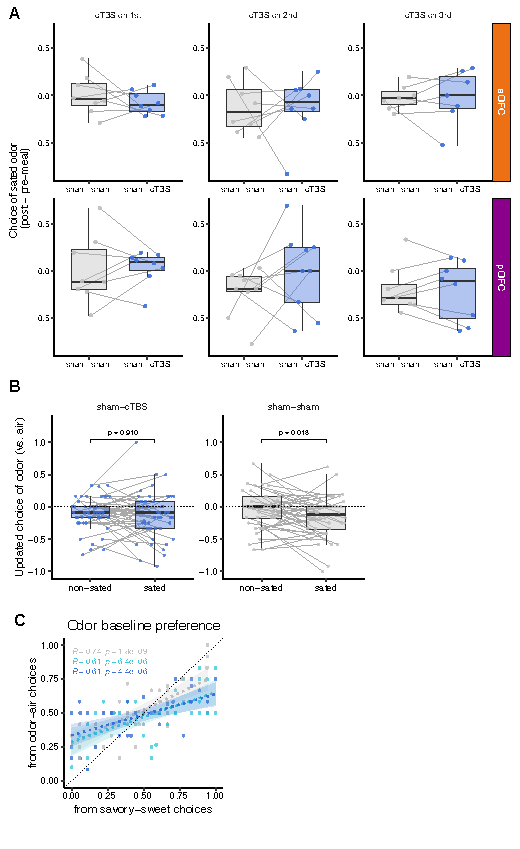
\includegraphics[width=0.7\linewidth]{EDfig_day2.pdf}
}{EDFig_day2} 



\extendeddatafigure[
\textbf{Supplementary results on cTBS effect on discrimination learning.} 
\textbf{A.} Change of response times across runs. 
\textbf{B.} Effect of cTBS on estimated learning rates, separated by Day 1 TMS order. 
\textbf{C.} Relationship between estimated learning rates and perceived TMS discomfort/intensity, separated by Day 1 TMS order.
]{
\includegraphics[width=0.7\linewidth]{EDfig_disc.pdf}
}{EDFig_disc}  



%%=============================================%%
%% For submissions to Nature Portfolio Journals %%
%% please use the heading ``Extended Data''.   %%
%%=============================================%%

%%=============================================================%%
%% Sample for another appendix section			       %%
%%=============================================================%%

%% \section{Example of another appendix section}\label{secA2}%
%% Appendices may be used for helpful, supporting or essential material that would otherwise 
%% clutter, break up or be distracting to the text. Appendices can consist of sections, figures, 
%% tables and equations etc.



%%===========================================================================================%%
%% If you are submitting to one of the Nature Portfolio journals, using the eJP submission   %%
%% system, please include the references within the manuscript file itself. You may do this  %%
%% by copying the reference list from your .bbl file, paste it into the main manuscript .tex %%
%% file, and delete the associated \verb+\bibliography+ commands.                            %%
%%===========================================================================================%%

\bibliography{references}% common bib file
%% if required, the content of .bbl file can be included here once bbl is generated
%%\input sn-article.bbl


\end{document}
